\documentclass[11pt, oneside]{article}    
%\usepackage{ijcai18}
%\usepackage{apacite}
\usepackage{geometry}
\geometry{letterpaper}
\usepackage{graphicx}
\usepackage{color}
\usepackage{xcolor}
\usepackage{amssymb}
\usepackage{hyperref}
\title{NIPS 2018 Competition proposal: Racial and Gender Bias in Face-based Attributes Analysis}
\author{Esube Bekele\thanks{The Leader organizer should be the first author of the proposal.} \and Joy Buolamwini \and Timnit Gebru \and Wallace Lawson 
    %\and Ian Goodfellow 
    %\and Samy Bengio 
    \\
{\tt esube.bekele.ctr@nrl.navy.mil}\\
}
\date{\today}

\makeatletter
    \let\@internalcite\cite
    \def\cite{\def\citeauthoryear##1##2{##1, ##2}\@internalcite}
    \def\shortcite{\def\citeauthoryear##1{##2}\@internalcite}
    \def\@biblabel#1{\def\citeauthoryear##1##2{##1, ##2}[#1]\hfill}
\makeatother

\begin{document}
\maketitle

\subsection{Overview of the competition}
% Summarize the background, available data, methods, available baseline, potential impact.
% Background and impact review

Despite recent success of face recognition and facial attributes  analysis systems, research suggests existence of a wide range of unintentional biases toward a specific racial or gender group \cite{phillips2011other} \cite{klare2012face}. Facial analysis is increasingly becoming pervasive in our daily lives for various applications such as face-based verification, identification, and criminal suspect profiling. More specifically, adoption by  law enforcement These biases have significant ramifications as these automated facial recognition and facial attributes analysis systems are widely adopted by law enforcement and other critical areas such as healthcare. Most common facial attributes in automated facial analysis include gender, race, and age \cite{fu2014learning} \cite{ng2015review} \cite{han2015demographic}. Face-based Gender and facial skin tone classification are covered in this competition.

% Availbale data review
Recent study of effect of demographics on facial gender classification showed this bias on three commercially available gender classification systems \cite{buolamwini2018gender}. As part of eliciting these biases, a new dataset was collected that is balanced in gender and skin tone type called Pilot Parliaments Benchmark (PPB). Although there are many publicly available face datasets that have race, gender, age,and other face-based attributes, we will primarily use this benchmark dataset for evaluation (as test set) in this competition.

% Methods and available baseline for each track
The competition will have two separate tracks. In the first track, researchers will be generating samples from existing datasets to illustrate such racial and gender biases in existing facial attributes analysis commercial systems and methods. In the second track, we will provide imbalanced dataset for race and gender and researchers will submit solutions that learn the facial attribute while minimizing the gender and racial bias in the classification performance.

\subsection{Keywords}
% Competition keywords, up to five, from generic to specific.
Other-race Effect, Automated Face Analysis, Gender Recognition, Bias in Facial attribute Analysis

\subsection{Novelty}
% (Have you heard about similar competitions in the past? If yes, describe the key differences. O/w disregard)
%Indicate whether this is a completely new competition, a competition part of a series, eventually re-using old data.
To the best of our knowledge this will be the first time such competition that is targeted at eliciting racial and gender biases in face recognition and analysis systems and solving these biases using techniques other than simply balancing the training dataset. Balancing datasets for every demographic group and gender is usually impractical for commercial applications with consequential impact such as watch-list surveillance \cite{kamgar2011toward} and person of interest identification \cite{best2014unconstrained}.

\section{Competition description}

\subsection{Background and impact}

% Provide some background on the problem approached by the competition and fields of research involved. Describe the scope and indicate the anticipated impact of the competition prepared (economical, humanitarian, societal, etc.). Justify the relevance of the problem to the targeted NIPS community and indicate whether it is of interest to a large audience or limited to a small number of domain experts (estimate the number of participants). A good consequence for a competition is to learn something new by answering a scientific question or make a significant technical advance.

% Extended Background
In psychology, there is a well documented phenomenon called "own-race" or "other-race" bias that people recognize faces and face related attributes of their own race better than that of other races \cite{furl2002face}. These inherent bias manifests itself in automated face recognition and analysis systems in part due to the unintentional imbalance in the datasets used to train such systems \cite{phillips2011other}. As shown in the Face Recognition Vendor Test (FRVT) by the National Institute of Standards and Technologies (NIST)  every four years, the performance of automated facial analysis has been steadily improving \cite{grother2010report}. The first breakdown of facial analysis systems performance by demographic groups \cite{phillips2011other} showed, however, that this performance improvement is not uniform across demographic groups of race and gender.

% Extended impact
With the wide spread adoption of automated facial analysis systems by law enforcement such as state and local police and federal immigration enforcement, proper regulation of such systems is of paramount importance. A recent report by Georgetown law school center on privacy and technology highlights the presence and consequences of racial bias embedded in such systems \cite{garvie2016perpetual}. The report indicated that 50\% (and expanding fast) of American adults are in a law enforcement face recognition network. It also highlights the dire consequences of such unregulated law enforcement face recognition showing such systems disproportionately affect African Americans as these systems are less accurate in identifying African Americans. Recent studies show the effect demographic groups on face analysis performance \cite{han2015demographic} \cite{farinella2012demographic} \cite{klare2012face}. Although these preliminary findings seem to suggest the existence of such bias and its potential consequences, there is dearth of research in this area to both find the source of such bias in facial analysis systems and solutions. 

% About the competition and relevant experience by authors
First, it is important to pinpoint whether such bias is primarily due to skin tone (race or ethnicity) and gender or these systems are exploiting other background information such as clothing and other visible attributes that correlate with specific demographic groups. Then, it is also important to solve this bias in facial analysis systems in the presence of imbalanced training dataset. Therefore, this competition has two tracks correspondingly. The first track requires users to use the PPB dataset and generate samples that elucidate the source of such bias in commercial face recognition software by manipulating the demographic dimensions of gender and facial skin tone. The original PPB dataset is balanced with respect to these demographics groups to avoid additional bias in the testing set \cite{buolamwini2018gender}. In the second track, we solicit submission that focus on a combination of novel and existing algorithms and architecture that result in relatively uniform performance across demographic groups. For this track, we will add additional samples as test set on top of the original PPB dataset. Esube has experience on data science competitions (with a master rank on kaggle.com) and we intend to use kaggle.com for hosting the competition. Joy and Timnit has collected and annotated the original PPB dataset.

\subsection{Data}
%If the competition uses an evaluation based on the analysis of data,
%please provide detailed information of the available data and
%their annotations, and, in case, what the data generation
%procedure will be (in this case, it must be clear in the document
%that the data will be ready prior to the official launch of the
%competition). Please justify that: (1) you have access to large
%enough datasets to make the competition interesting and draw
%conclusive
% results; (2) the data can be made freely available;(3) the ground truth has been kept confidential.

Demographic imbalances in existing face-based gender recognition datasets led to creating a new dataset for gender classification called the Pilot Parliaments Benchmark (PPB) \cite{buolamwini2018gender}. This dataset will be primarily used as an evaluation set for first track of the competition. The dataset is composed of 1270 identities (1 image/subject) from 3 African (Rwanda, Senegal, and South Africa) and 3 European countries'(Iceland, Finland, Sweden) national parliaments. Fig. \ref{fig_ppb} shows representative samples and average images from each country and gender. Table \ref{ppb} summarizes the PPB dataset statistics compared to recent face recognition benchmarks.

\begin{figure}[t]
    \label{fig_ppb}
    \centering
    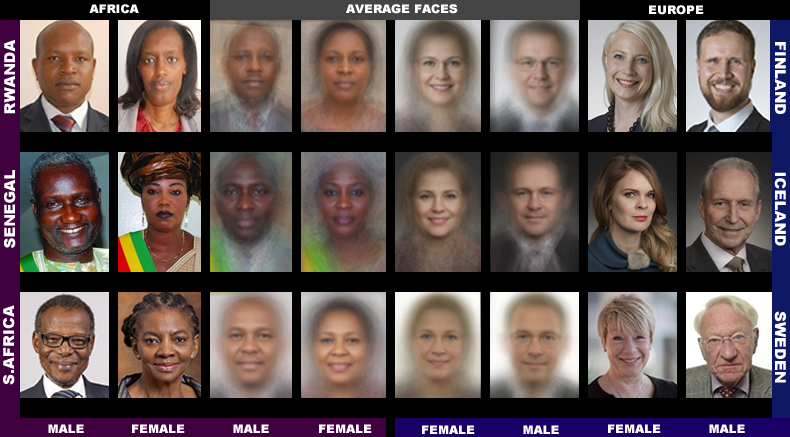
\includegraphics[width=140mm]{fig/ppb}
    \caption{Sample images and average faces from each country and gender in the PPB dataset.}
\end{figure}

\begin{table}[b]
    \caption{Dataset statistics of PPB compared to IJB-A and Adience face recognition benchmarks}
    \label{ppb}
    \centering
    \begin{tabular}{cccc}
        
        \hline
        feature & PPB & IJB-A & Adience \\
        \hline
        Release Year & 2017 & 2015 & 2014 \\
        \# of Subjects & 1270 & 500 & 2284 \\
        Avg. IPD (in pixels) & 63 & - & - \\
        BBox Size & 141 (avg) & $\geq$ 36 & - \\
        Image Width & 160-590 & - & 816 \\
        Image Height & 213-886 & - & 816 \\      
        \hline
    \end{tabular}
\end{table}


The major defining characteristics of facial analysis and recognition benchmark datasets is their imbalance with respect to racial/ethnic and gender demographic groups \cite{phillips2011other, han2015demographic}. The PPB dataset is intentionally balanced in these demographic groups to allow a balanced evaluation of facial analysis algorithms (see Table \ref{skin_ton}). This balance in the test dataset (PPB) sets equivalence across the demographic groups in all the metrics evaluated. 

\begin{table}[b]
    \caption{Facial skin ton and gender breakdown of the dataset PPB compared to IJB-A and Adience}
    \label{skin_ton}
    \centering
    \begin{tabular}{cccc}
        
        \hline
        Demographics Group & PPB & IJB-A & Adience \\
        \hline
        Darker Female & 21.3\% & 4.4\% & 7.4\% \\ 
        Darker Male & 25.0\% & 16.0\% & 6.4\% \\
        Lighter Female & 23.3\% & 20.2\% & 44.6\% \\
        Lighter Male & 30.3\% & 59.4\% & 41.6\% \\       
        \hline
    \end{tabular}
\end{table}

For the second track of the competition, we will use the CelebA dataset \cite{liu2015deep} as training set and the PPB dataset as test for gender classification. While CelebA is a large unconstrained images of faces in the wild, PPB is a more balanced and constrained, in terms of pose and illumination, evaluation benchmark. CelebA contains 10,000 identities with 20 images each on average for a total of 202,599 images labeled with 40 attributes and 5 key points. The attributes include gender and skin color (only for pale skin) and hair color. Hence, it represents a typical imbalanced and unconstrained training set for facial analysis.

For the first track, we will release half of the African and half of the European set of images for a total of 634 images as part of the development package to generate morphed images by manipulating the skin ton and gender dimensions. We reserve the remaining 636 images for the second track again released as part of the development package. We plan to expand this test set by adding additional labeled images of national parliamentarians from other (but equivalent in terms of skin type and gender labels) countries for the final test sets of each track. 

\subsection{Tasks and application scenarios}

%Describe the tasks of the competition and explain to which specific real-world scenario(s) they correspond to. If the competition does not lend itself
%to real-world scenarios, provide a justification. Justify that the problem posed are scientifically or technically challenging but not impossible to
%solve. If data are used, think of illustrating the same scientific problem using several datasets from various application domains.

This competition will have two separate tasks that are divided into two separate tracks. Competition participants are free to submit to both tracks. 

\subsubsection{Commercial Face Analysis Systems Challenge}
In this challenge participants are required to evaluate the performance of three commercial face-based gender classification systems (Microsoft, IBM, and Face++) with respect to the skin tone continuum. The main purpose of this challenge is to show the effect of skin type on gender classification. This is analogous to generating adversarial examples but constrained only by changing only the skin type. This challenge helps to pinpoint whether demographics (specifically skin type in this case) alone influence performance of gender classifiers and to rule out other confounding factors such as visible portions of clothing that would correlate with these specific demographic groups.

In this track, each participant will be given 634 images of the PPB dataset as part of a development kit that also contains tools for cross validation, pre-trained gender classifiers, links to the commercial face analysis cloud-based tools and evaluation performance metrics. For each image in the development package, each participant is expected to generate new image that is similar to the original image in identity. The only modification allowed to the input images are manipulating the skin tone of the subject in the image using any face morphing or feature-level facial attribute manipulation models. 

The final performance in this challenge will be evaluated with a separate test set of images from parliamentarians from other countries to minimize over-fitting. In this task participants are prohibited to perform any adversarial manipulation on the image to get lower score other than the skin tone manipulation. Submission that results in the lowest performance in metrics as described in the metrics section will be winners.
 
\subsubsection{Face-based Gender Recognition Challenge}
This second task is aimed at training gender recognition models with unconstrained non-balanced realistic dataset to have balanced performance in each of the four course demographic categories. For this purpose, each participant will be required to train a model (or ensemble of models) on CelebA dataset. Participants are allowed to use all the 39 attribute labels as long as it helps improve the gender classification. For instance, they could use the "Pale\_skin" attribute to categorize the images based on skin lightness and use sample weights during training. Participants are allowed to employ any architecture, training technique, data augmentation (no external dataset is allowed), output probability calibration and other methods for training on imbalanced dataset.

We will release 636 images of the PPB dataset with the development kit for local cross validation and testing. We will collect and annotate new set of final test set images of parliamentarians from other countries than the original six countries in the original PPB dataset to avoid over-fitting. 

In both tracks of the competition, participants are required to submit their code as part of their submission by the deadline date to be considered for the first three top position.


\subsection{Metrics}

%For quantitative evaluations, select a scoring metric and justify
%that it effectively assesses the efficacy of solving the problem
%at hand. It should be possible to evaluate the results
%objectively. If no metrics are used, explain how the evaluation
%will be carried out.

\subsection{Baselines and code available}

%Specify what are (will be) the baselines for the competition, and
%whether there is available code for participants (e.g., a starting
%kit) and evaluation. Provide preliminary results, if available.

\subsection{Tutorial and documentation}

%Provide a reference to a white paper you wrote describing the
%problem and/or explain what tutorial material you will provide.


\section{Organizational aspects}
\subsection{Protocol}

%Explain the procedure of the competition: what the participants will have to do, what will be submitted (results or code), and the evaluation procedure.
%Will there be several phases? Will you use a competition platform with on-line submissions and a leader board? Indicate means of preventing cheating.
%Provide your plan to organize beta tests of your protocol and/or platform.

Each track of the competition will have preliminary rounds of up to 5 submissions maximum and a final round submission. The preliminary rounds are for the purpose of giving participants feedback other than their local internal validation using the preliminary test sets released together with the development kit. The final round will be scored on the private test set and only this final round of submissions are considered for ranking teams. 

We plan to apply for hosting research based competition with kaggle.com. It has self contained on-line submission and leader boards.

\subsubsection{Preliminary Rounds}

For the commercial face-based gender recognition systems evaluation track, we will release 634 random images from the PPB split by countries for internal cross validation and preliminary rounds submissions. The protocol for the preliminary rounds of this track are as follows.

\begin{enumerate}
    \item Participants are expected to generate a new sample for each of the 634 images in the development kit and submit the generated image. Participants are allowed to use their own image manipulation models or traditional pipeline. But, no commercial software is allowed.
    \item Organizers will only score the newly generated images on the three commercial face-based gender recognition systems and performance metrics for each vendor and average performance metrics will be released for the participants. At this stage, organizers will not check for cheating.
\end{enumerate}

For the face-based gender recognition challenge, participants will follow the following protocols.

\begin{enumerate}
    \item Organizers will release 636 random images from the PPB evaluation benchmark as part of the development kit.
    \item Participants are expected to train their face-based gender recognition models on CelebA dataset. The aligned and cropped versions of the CelebA dataset together with 40 attributes (gender is one of these attributes) will be made available both on the competition site and kaggle.com. Submissions are encouraged that exploit and submit predictions of attributes of CelebA other than gender to help in balanced gender recognition in a multi-label classification. But, only the gender prediction will be used to score submissions.
    \item Organizers will score the submissions on the 636 preliminary round test sets and release the gender recognition performance to participants (in the form of public leader board).
\end{enumerate}

\subsubsection{Final Rounds}
For the final round we will set aside 1000 images and their skin type and gender labels for scoring the final submissions. To prevent cheating in this final round, the following protocols are followed:

\begin{itemize}
    \item The labels for the final round images are held confidentially and will not be made available until the competition ends and winners are announced. The images will be released 
    \item All participants will have to submit their code or open source it on github and submit a link to it to be considered for the top 3 positions. Submissions without source code in the final round will not be scored.
    \item For the first track of this competition, organizers will make at most care to run the code and generate new samples for the 1000 final test images. Special care will be taken for the top 3 teams to make sure that their code is not generating any adversarial samples other than skin tone manipulation in an effort to exploit adversarial vulnerability of these commercial gender recognition systems. After the skin tone manipulation, the original image and the generated image will not be $L_{\infty}$ consistent and hence it is difficult to check if there is added adversarial attack on the generated images.
    \item For the gender recognition challenge track, organizers will run the classification code submitted by participants on the 1000 images and score them against their labels. 
\end{itemize}


In this final round, the protocol for each track is as follows. 

\begin{enumerate}
    \item For both tracks of the competition, participants are required to submit their code by the competition deadline.
    \item Organizers will run the source code on the 1000 final round test images and generate manipulated images and evaluate the three commercial systems with them in the case of the first track. For the second track, organizers will run the code and generate gender predictions and score them against the ground truth gender labels.
    \item Organizers determine the top 3 teams in each track. 
    \item For the first track, the top 3 submissions are selected based on performance metrics for each vendor and average lowest performance metric for each of the two demographic groups (i. e., dark skin type male and dark skin type female).
    \item The top three teams source code will be carefully examined to make sure adversarial attacks are not injected together with the skin tone manipulation.
    \item For the second track, the top 3 teams are selected based on the highest balanced performance metrics for all the four demographic groups.
    \item Organizers will announce the results and release the final round 1000 test images and their labels. Organizers will combine the new 1000 test images with the original PPB dataset so that further research and commercial systems will use this as evaluation benchmark test sets for gender and race balanced facial analysis.
\end{enumerate}


\subsection{Rules}

%Provide a list of special rules. 
%For qualitative evaluations (e.g. demonstration competitions), select a committee and prepare guidelines for the committee.
\begin{enumerate}
    \item Anyone can participate with the exception of the organizers and anyone that has any conflict of interest with the organizers.
    \item To be eligible for scoring in the final rounds, participants are required to submit their source code or open source it on github.
    \item Source code must not produce any errors or the submission will be abandoned without scoring.
    \item Participants are required to submit clear documentation of their code on how to run it on the final round test images. The documentation also should clearly list set of dependencies for the code.
    \item Any leader board probing will not be allowed and will be grounds for elimination from the competition.
    \item No external dataset is allowed. Only the CelebA dataset and PPB dataset released by the organizers are allowed for this competition.
    \item No pre-training other than ImgaeNet pre-trained models is allowed in this competition.
\end{enumerate}

\subsection{Schedule}

%Provide a time line for competition preparation and for running the competition itself. Propose a reasonable schedule leaving enough time for the organizers
%to prepare the event (a few months), enough time for the participants to develop their methods (e.g. 90 days), enough time for the organizers to review the entries, analyze and publish the results. 
The proposed competition schedule is as follows.

{\it April 1st, 2018} {\bf Start of competition promotion}: Start of Competition Promotion. We will launch the competition website with the call for submissions. Start heavy promotion of the competition via social media, at upcoming conferences and mailing lists.

{\it June 30th, 2018} {\bf Release of development kit and official start of the competition}: The competition starts with the release of the development kit. 

{\it June 30th, 2018 - October 1st, 2018} {\bf Duration of the competition}: Submissions are allowed starting this date until the competition closes for a maximum of 5 preliminary round of submission by each team for each track.

{\it October 1st, 2018} {\bf Deadline for the final round}: Each team will have one more final round submission which is due on October 1st, 2018.

{\it October 1st 2018 - October 30th, 2018} {\bf Final round evaluation}: We will evaluate final round submissions on the separate test images that are not publicly released.

{\it November 1st 2018} {\bf Announcement of winners}: Winners (top 3 teams) in each track will be announced and the final round test images will be made public.

\subsection{Competition promotion}

%The plan that organizers have to promote participation in the competition (e.g., mailing lists in which the call will be distributed, invited talks, etc.).
This competition will be promoted using the organizers' Facebook, Twitter, Reddit and other social media accounts and pages, and mailing lists. Moreover, we encourage black professionals in AI to take part in this competition. To this effect, we will heavily promote it in the Black in AI Facebook group and discussion forums and we wish winners of both tracks to present in the next Black in AI workshop which will be co-located with NIPS 2018.

\subsection{Organizing team}

%Provide a short biography of all team members, stressing their competence for their assignments in the competition organization. Make sure to include: coordinators, data providers, platform administrators, baseline method providers, beta testers, and evaluators.
{\bf Esube Bekele}: is a National Research Council Fellow at the US Naval Research Lab (NRL) in the Navy Center for Research in Applied Artificial Intelligence (NCRAAI). Esube has extensive experience in data science kind of competitions and he currently serves in the organizing team od DC Data Science (Large meetup for data science professions in the Washington, DC area). Currently, he holds a master rank at kaggle.com. Esube will serve as the primary coordinator of the competition providing data, development kit, platform administration, baseline methods and evaluation performance metrics--all with in the scope of his regular work as fellow at NRL.

{Joy Boulamwini}: 

{Timnit Gebru}:

{Wallace Lawson}:

%{Ian Goodfellow}:

%{Samy Bengio}:

\section{Resources}
\subsection{Existing resources, including prizes}

%Describe your resources (computers, support staff, equipment, sponsors, and available prizes).
We hope to host the competition at kaggle.com similar to last year's NIPS competition on adversarial examples. We do not plan to provide monetary prizes. However, top 3 submissions in each track will be invited to present in Black in AI workshop, which will be collocated with NIPS 2018 and this competition track of NIPS 2018.

%% The file named.bst is a bibliography style file for BibTeX 0.99c

\bibliographystyle{named}
%\bibliographystyle{apacite}
\bibliography{egbib}

\end{document}
